\chapter{序论}
\thispagestyle{empty}

\setlength{\fboxrule}{0pt}\setlength{\fboxsep}{0cm}
\noindent\shadowbox{
\begin{tcolorbox}[arc=0mm,colback=lightblue,colframe=darkblue,title=学习目标与要求]
\kai\textcolor{darkblue}{1.~~了解科学计算的一般过程.}\\
\kai\textcolor{darkblue}{2.~~了解数值计算方法的研究内容和特点.}\\
\kai\textcolor{darkblue}{3.~~理解数值计算误差的有关概念.}\\
\kai\textcolor{darkblue}{4.~~掌握数值计算误差的控制方法.}
\end{tcolorbox}}
\setlength{\fboxrule}{1pt}\setlength{\fboxsep}{4pt}

\section{Colored boxes}

\begin{tcolorbox}[colback=red!5,colframe=red!75!black]
  My box.
\end{tcolorbox}

\begin{tcolorbox}[colback=blue!5,colframe=blue!75!black,title=My title]
  My box with my title.
\end{tcolorbox}

\begin{tcolorbox}[colback=green!5,colframe=green!75!black]
  Upper part of my box.
  \tcblower
  Lower part of my box.
\end{tcolorbox}

\begin{tcolorbox}[colback=yellow!5,colframe=yellow!75!black,title=My title]
  I can do this also with a title.
  \tcblower
  Lower part of my box.
\end{tcolorbox}

\begin{tcolorbox}[colback=yellow!10,colframe=red!75!black,lowerbox=invisible,
  savelowerto=\jobname_ex.tex]
  Now, we play hide and seek. Where is the lower part?
  \tcblower
  I'm invisible until you find me.
\end{tcolorbox}

\begin{tcolorbox}[colback=yellow!10,colframe=red!75!black,title=Here I am]
  \input{\jobname_ex.tex}
\end{tcolorbox}


\begin{tcolorbox}[colback=blue!50,colframe=blue!25!black,coltext=yellow,
    fontupper=\Large\bfseries,arc=6mm,boxrule=2mm,boxsep=5mm]
  Funny settings.
\end{tcolorbox}

\subsection{\LaTeX-Table}

\begin{table}[h]\begin{center}\color{darkblue}\caption{计算结果}\color{black}\label{tab1-2}
{\footnotesize
\begin{tabular}{r|r||r|r||r|r||r|r}\arrayrulecolor{darkblue}\hline\rowcolor{lightblue}
  $n$&$I_n$&$n$&$I_n$&$n$&$I_n$&$n$&$I_n$\\\hline
  19&0.008\ 3&14&0.011\ 2&9&0.016\ 9&4&0.034\ 3\\
  18&0.008\ 9&13&0.012\ 0&8&0.018\ 8&3&0.043\ 1\\
  17&0.009\ 3&12&0.013\ 0&7&0.021\ 2&2&0.058\ 0\\
  16&0.009\ 9&11&0.014\ 1&6&0.024\ 3&1&0.088\ 4\\
  15&0.010\ 5&10&0.015\ 4&5&0.028\ 5&0&0.182\ 3\\\hline
 \end{tabular}}\end{center}\end{table}


\section{\LaTeX-Examples}

\begin{tcblisting}{colback=red!5,colframe=red!75!black}
This is a \LaTeX\ example:
$\displaystyle\sum\limits_{i=1}^n i = \frac{n(n+1)}{2}$.
\end{tcblisting}


\section{Theorems}

\begin{defi}{Summation of Numbers}{defi1.1}
  For all natural number $n$ it holds:\\[2mm]
  $\displaystyle\sum\limits_{i=1}^n i = \frac{n(n+1)}{2}$.
\end{defi}

\begin{theo}{Summation of Numbers}{theo1.1}
  For all natural number $n$ it holds:\\[2mm]
  $\displaystyle\sum\limits_{i=1}^n i = \frac{n(n+1)}{2}$.
\end{theo}

\begin{coro}{Summation of Numbers}{coro1.1}
  For all natural number $n$ it holds:\\[2mm]
  $\displaystyle\sum\limits_{i=1}^n i = \frac{n(n+1)}{2}$.
\end{coro}
We have given Theorem \ref{Theorem:theo1.1} on page \pageref{Theorem:theo1.1}.



\begin{table}[h]\begin{center}\color{darkblue}\caption{计算结果}\color{black}\label{tab1-1}
{\footnotesize
\begin{tabular}{r|r||r|r||r|r||r|r}\arrayrulecolor{darkblue}\hline\rowcolor{lightblue}
  $n$&$I_n$&$n$&$I_n$&$n$&$I_n$&$n$&$I_n$\\\hline
  1&0.088\ 4&6&0.034\ 4&11&-31.392\ 5&16&9.814\ 5e+4\\
  2&0.581\ 0&7&-0.029\ 0&12&157.045\ 7&17&-4.907\ 3e+5\\
  3&0.043\ 1&8&0.270\ 1&13&-785.151\ 6&18&2.453\ 6e+6\\
  4&0.347\ 0&9&-1.239\ 3&14&3.925\ 8e+3&19&-1.226\ 8e+7\\
  5&0.026\ 5&10&0.296\ 7&15&-1.962\ 9e+4&20&6.134\ 1e+7\\\hline
\end{tabular}}\end{center}\end{table}

\section{graphicx}

\begin{figure}[h]
\begin{minipage}[t]{0.5\linewidth}
\centering
\includegraphics[totalheight=1.2in]{fig/tu2-2}
\caption{不动点迭代法收敛} \label{fig:tu2-2}
\end{minipage}

\begin{minipage}[t]{0.5\linewidth}
\centering
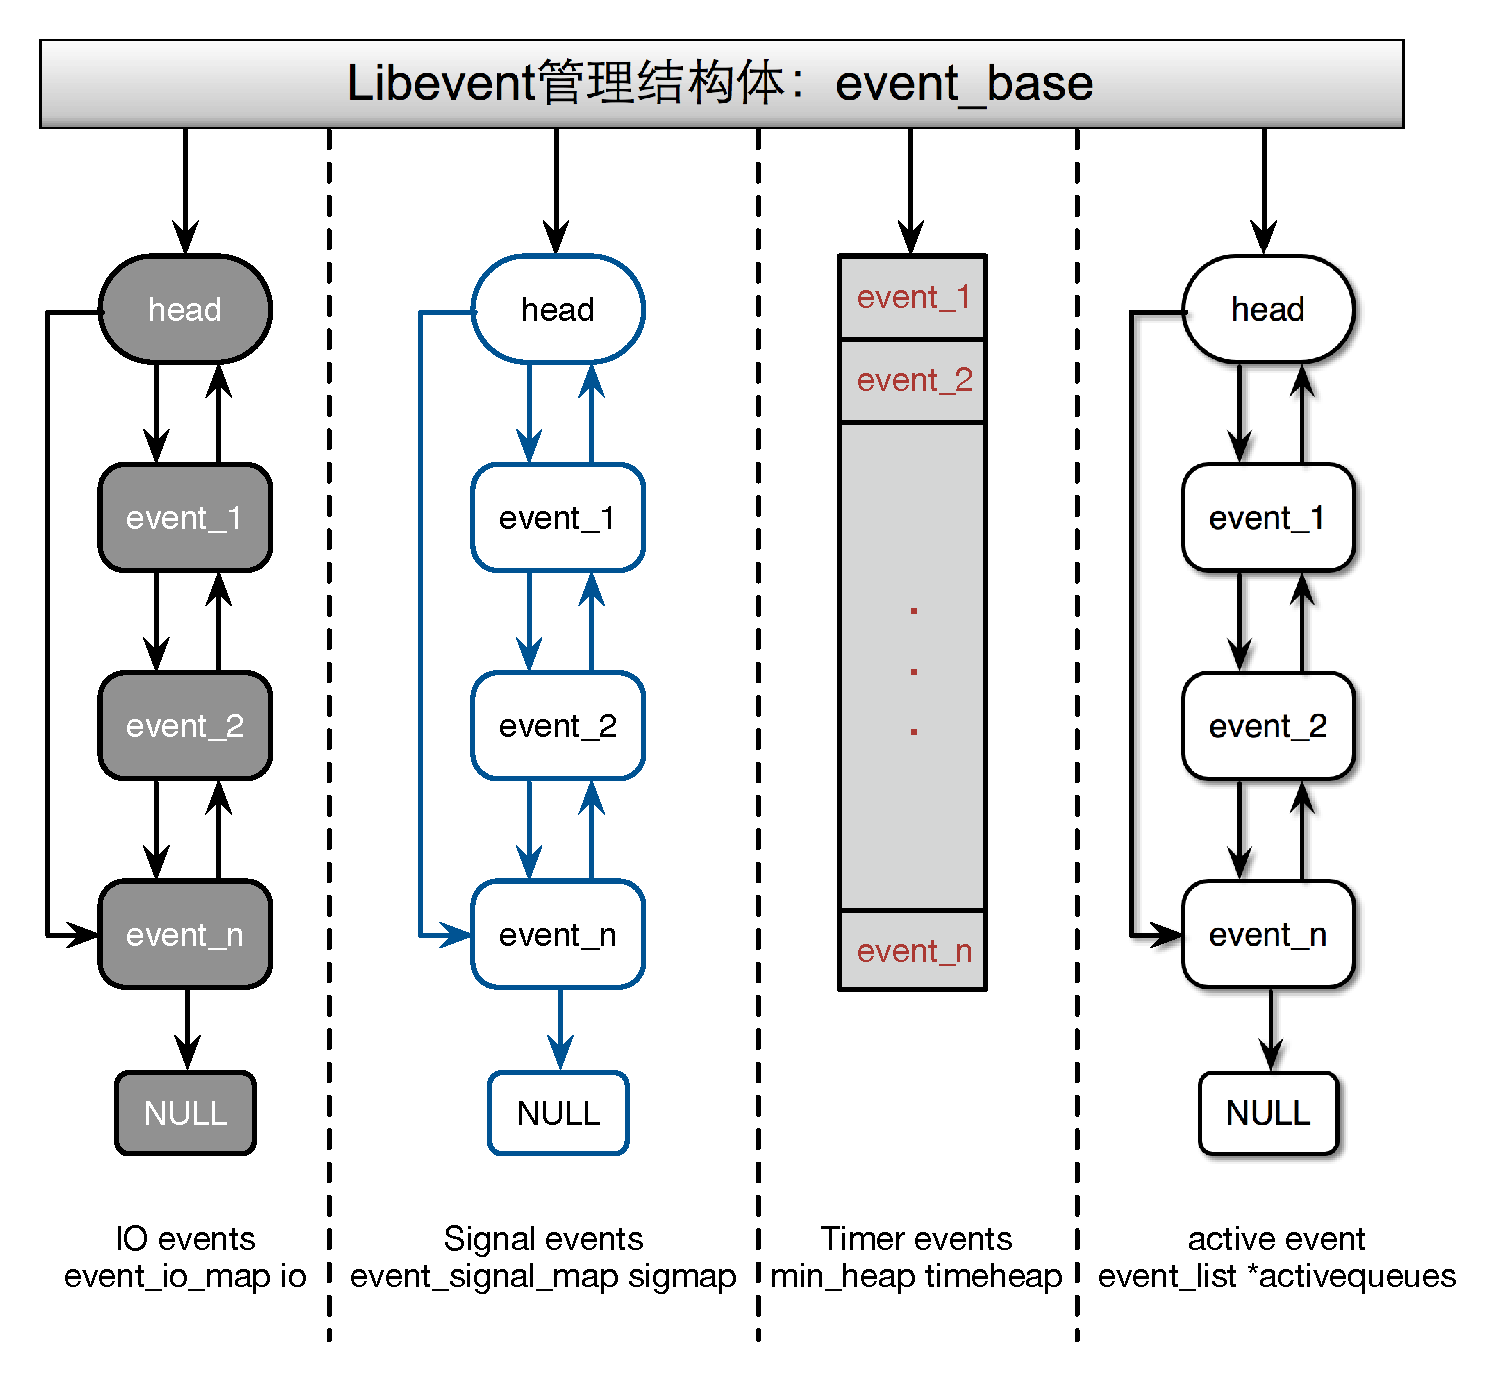
\includegraphics[totalheight=1.3in]{fig/tu2-3}
\caption{不动点迭代法发散} \label{fig:tu2-3}
\end{minipage}
\end{figure}



\vspace{0.5cm}
\addcontentsline{toc}{section}{\protect\numberline{}{习题一}}
\markboth{习题一}{习题一} \centerline{\textcolor{black}{\hei{\normalsize 习题一}}}\vspace{0.5cm}


